\documentclass[11pt, oneside]{article} 
\usepackage{geometry}
\geometry{letterpaper} 
\usepackage{graphicx}
	
\usepackage{amssymb}
\usepackage{amsmath}
\usepackage{parskip}
\usepackage{color}
\usepackage{hyperref}

\graphicspath{{/Users/telliott_admin/Dropbox/Tex/png/}}
% \begin{center} 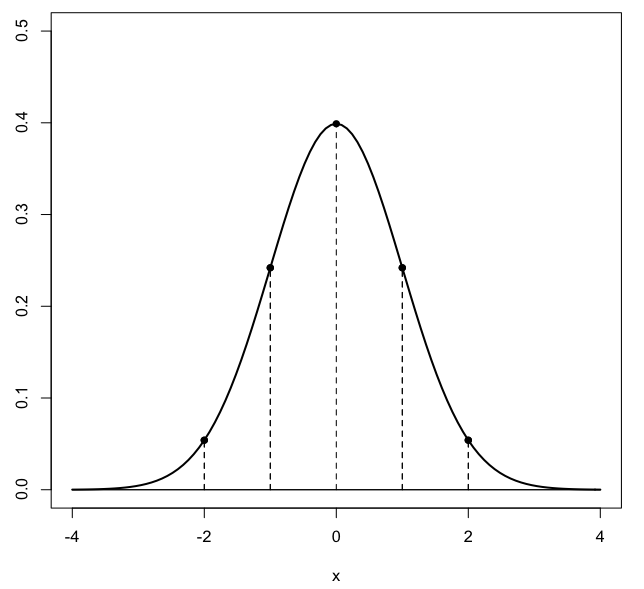
\includegraphics [scale=0.4] {gauss3.png} \end{center}

\title{Escape from earth}
\date{}

\begin{document}
\maketitle
\Large

In this chapter, we will calculate the energy required to move a body which is initially at some distance $r_1$ from the center of the earth (say, $R$, the earth's radius), to a position at some other distance $r_2$.

Eventually, we will consider problems related to the orbits of planets around the sun.  But let's start with idealized circular orbits and consider escape velocity which does not require vector calculus to solve.

\subsection*{gravitational potential}

First, suppose you stand on the earth's surface and throw a ball straight up into the air with a velocity $v$.  It reaches some maximum height where its vertical velocity is zero.  It has traded kinetic energy for potential energy.  Be sure to move out of its way as it comes down.

Potential energy due to gravity increases with height above the earth.

Suppose we climb the steps up to the top of the leaning Tower of Pisa and then drop a marble over the edge.  At the start the marble has zero velocity and at the end it has some velocity which we can calculate, neglecting air resistance.  

We have the basic equation of motion with acceleration
\[ y = \frac{1}{2}at^2 + v_0 t + y_0 \]
and its time-derivative
\[ v = \frac{dy}{dt} = at + v_0 \]
We can obtain a formula that does not involve the time
\[ v^2 - v_0^2 = 2a (y - y_0) \]

Do this by starting with equation 1 and rearranging:
\[ 2(y - y_0) = at^2 + 2v_0 t \]
then solve equation 2 for $t = (v - v_0)/a$ and substitute
\[ 2(y - y_0) = a\frac{(v - v_0)^2}{a^2} + 2v_0 \frac{v - v_0}{a} \]
\[ 2a(y - y_0) = (v - v_0)^2 + 2v_0(v - v_0) \]
\[ = v^2 - v_0^2 \]
For gravity
\[ v^2 - v_0^2 = -2g (y - y_0) \]

We write the sign of the acceleration as negative, that is, $- g$, where it's understood that $g > 0$.  

The usual choice is to have the coordinate system point up.  If the ball is over my head, then $|v| < |v_0|$ (both going up and coming down), so the left-hand side is negative, which matches $y > y_0$ only if the sign on the acceleration is minus.  

Later, when we calculate work, in some cases, the relevant force will be the one which we have applied to oppose gravity, and that force points up.

Call the distance $y - y_0 = h$.  Then
\[ v^2 - v_0^2 = - 2gh \]
At the top, $v = 0$
\[ v_0^2 = 2gh \]
This gives
\[ \frac{1}{2} mv_0^2 = mgh \]

Which you probably recognize.  At a height $h$ above the ground there is a potential energy difference of $mgh$.  After dropping through a height $h$, all this potential energy is converted to kinetic energy $mv^2/2$.
\[ v^2 = 2gh \]
\[ v = \sqrt{2gh} \]

\subsection*{escape velocity}

Now, imagine an object starting from rest on the surface of the earth and then giving it enough velocity in an idealized trajectory (simply the vertical direction) so that it can move far enough away to be free from gravity altogether.  In this problem the force decreases as the object moves away.

A simple approach is to use the principle of conservation of energy:  we will impart enough kinetic energy so that the increase in potential energy after the motion is just balanced.  The question is how to compute the potential energy.

Later on, in vector calculus we will use this expression for work
\[ W = \int_C \mathbf{F} \cdot d \mathbf{r} \]

We must use an integral because the force is a function of $r$, and we use the dot product because the force and the changing position vector are not always aligned.

The work done over the course of the motion (force times distance) is equal to the energy added to the object.  The vector equation says that only the component of the force in the same direction as the motion contributes.

Luckily, we don't need to use a vector equation for this problem.  Just place the center of the earth at the origin, and treat all of the mass of the earth as being at that point.  (We will develop Newton's proof of this later, see \hyperref[sec:Newton_point_mass]{\textbf{here}}). 

Then, consider the force and motion as occurring only in one direction.  While $x$ or $y$  could be used for the variable, the conventional choice is $r$.  All of the (scalar) force and motion is in the $r$ direction.

In the vector approach, we learn that the force $\mathbf{F}$ is the gradient of a scalar function (called the potential energy)
\[ \mathbf{F} = - \nabla U \]

In 1D this just amounts to doing the scalar integral.

The usual derivation is that the change in potential energy in going from configuration $a$ to $b$, is minus the work done in going from $a$ to $b$ where
\[ W_{ab} = \int_a^b F(r) \  dr \]
and then
\[ \Delta U = U_b - U_a = - W_{ab} \]

For the first example above, we have $F = -mg$ and so
\[ W = \int_0^h -mg \ dy = -mgh \]
(Gravity does work on an object when it falls in the gravitational field, it does negative work on the object as it rises).  Then
\[ \Delta U = mgh \]

For the second case, where the change is large enough that the force is not constant, we write $F(r)$
\[ F(r) = - \frac{GmM}{r^2} \]
\[ W_{ab} = \int_a^b - \frac{GmM}{r^2} \ dr \]
\[ = \frac{GmM}{r} \ \bigg |_a^b \]
\[ = GmM \ [ \frac{1}{r_b} - \frac{1}{r_a} \ ] \]
then
\[ \Delta U = U_b - U_a = -W_{ab} \]
\[ = GmM \ [ \frac{1}{r_a} - \frac{1}{r_b} \ ] \]

We pick a convenient reference point, namely $ b \rightarrow \infty$.  The upper bound of $\infty$ makes this an \emph{improper} integral.  We say "oh we're not really going to infinity, just really far away, and then wonder, what would happen if we did go to infinity."

We also agree that this configuration is defined to have zero potential energy.  Then
\[ U_b - U_a = GmM \ [ \frac{1}{r_a} - \frac{1}{r_b} \ ] \]
\[ -U_a = \frac{GmM}{r_a}  \]
\[ U_a = -\frac{GmM}{r_a}  \]

If we're thinking about the potential due to gravity, the force points toward the earth.  The potential energy is larger the further away from earth you go, and is largest at infinity, where by definition it is equal to zero.  Thus, all other potential energies are negative.  To be on earth is, in that sense, to be trapped, since it requires an input of energy to lift you to some larger $r$ and less negative $U$.

This is, in magnitude, equal to the work we would have to do pitting some force against gravity to lift a mass $m$ to completely escape from the earth's gravity.  The larger the starting radius the less work there is to do.  Another way to state this is that the extra potential energy at some radius $r_1 > r_2$ is exactly equal to the work required to move between these points.

How much kinetic energy do we need to impart?  Using the standard form for K, we obtain this expression, valid for the earth's surface:
\[ \frac{1}{2}mv^2 = \frac{GM}{R} m \]
\[ \frac{1}{2}v^2 = \frac{GM}{R} \]
\[ v = \sqrt{ \frac{2GM}{R}} \]

The velocity needed is independent of the object's mass (though of course it will take more energy to get a bigger object from zero up to a certain velocity).  This velocity is called the escape velocity.

If we recall that the acceleration due to gravity at the surface of the earth is
\[ g = \frac{GM}{R^2} \]
substituting
\[ v = \sqrt{2gR} \]

We need to watch the units.  

If we use English (Imperial) units, $a = 32$ feet per sec$^2$.  $R = 3959$ miles, and in feet that is $3959 \cdot 5280$.  Hence $v = \sqrt{2 \cdot 32 \cdot 3959 \cdot 5280} \approx 36500$ feet per second.  

$15$ miles per hour is exactly equal to $22$ feet per second.
\[ 15 \ \frac{\text{miles}}{\text{hour}} \cdot 5280 \ \frac{\text{feet}}{\text{mile}} \cdot \frac{1}{3600} \ \frac{\text{hour}}{\text{second}} =  22 \ \frac{\text{feet}}{\text{second}} \]

The velocity works out to about $24,900$ miles per hour.  That's a lot.  A point on the equator of the earth rotates $24,900$ miles a day.

In MKS units, $a = 9.8$ meters per sec$^2$ and the earth's radius is $6371$ km so 
\[ v = \sqrt{2aR} \]
\[ = \sqrt{2 \cdot 0.0098 \cdot 6371} \]
\[ \approx 11.2 \ \frac{\text{km}}{\text{sec}} \]

The energy required to achieve a stable orbit around the earth has two parts:  a radial part that gives the needed potential energy and a tangential part that gives the necessary orbital velocity.  In the next chapter we will look at orbital velocities.  

\subsection*{Kline}

Morris Kline uses a different approach.  We start with the acceleration due to gravity whose absolute value is
\[ a = \frac{GM}{r^2} \]

You might think we should write this with a minus sign because $a$ points down, while $r$ increases going up.  However, as we said before, this is not correct.  The reason is that the force that must be exerted to escape from gravity points \emph{up}.

Write this explicitly as the second derivative of position with respect to time
\[ a = \frac{d^2 r}{dt^2} = \frac{GM}{r^2} \]

Now, he says, we'd like to integrate both sides (with respect to $t$, naturally).  That would give us $v(t)$ on the left.  But what is written on the right is not explicitly a function of time.  What to do?  

Use the chain rule!

Manipulating the left-hand side:

\[ \frac{d^2 r}{dt^2} = \frac{dv}{dt} = \frac{dv}{dr} \frac{dr}{dt} = v \frac{dv}{dr} \]

Clever, eh?  Hence
\[ v \frac{dv}{dr} = \frac{GM}{r^2} \]

Moving $dr$ to the right-hand side and integrating, we obtain
\[ \frac{v^2}{2} = -\frac{GM}{r} + C \]

You may recognize a connection between kinetic and potential energy here, we are just missing the mass $m$.

We can evaluate the constant $C$ by recognizing that we want $v=0$ for some particular $r$ that we're going to choose.  It may be $r \rightarrow \infty$ as we had above, or it might be some other $r$.  

What we could do is just to deal with the velocity and the radius at the two points, subtract, and then the constant goes away.
\[ \frac{v_2^2}{2} -  \frac{v_1^2}{2} = - \ [ \ \frac{GM}{r_2} - \frac{GM}{r_1} \ ]  \]

Let's call the radius where $v=0$, $r_{1}$.  There

\[ 0 = \frac{GM}{r_{1}} + C \]
\[ C = -\frac{GM}{r_{1}}  \]
\[ \frac{v^2}{2} = \frac{GM}{r} -\frac{GM}{r_{1}} \]

Now ask what happens in the limit as $r_1 \rightarrow \infty$, and the $r$ of interest to us is the radius of the earth $R$

\[ \lim_{r_1 \rightarrow \infty}  \frac{GM}{r_1} = 0 \]
\[ \frac{v^2}{2} = \frac{GM}{R}  \]

and this is the same result as we had before.

\subsection*{Kline II}

Kline also uses a different argument to achieve the same goal.
\[ \frac{d^2 r}{dt^2} = -\frac{GM}{r^2} \]

Multiply both sides by 
\[ \frac{dr}{dt} \cdot \frac{d^2 r}{dt^2} = -\frac{GM}{r^2} \cdot  \frac{dr}{dt} \]

The derivative is just a function.  Pretend we don't know what it is, call it $u$, and substitute the left-hand side \emph{only}.
\[ u = \frac{dr}{dt} \]
\[ u \ \frac{du}{dt} = -\frac{GM}{r^2} \cdot  \frac{dr}{dt} \]

Now, multiply by $dt$ and integrate.  Or if you prefer, reverse the chain rule and integrate both sides with respect to $t$.
\[ \frac{1}{2} u^2 =  \frac{GM}{r} + C \]

Recall that $u$ is really just $v$
\[  v = \frac{dr}{dt} = u \]
\[ \frac{1}{2} v^2 =  \frac{GM}{r} + C \]

A bit of sleight of hand.

\end{document}  